\chapter{Implementation}

\setlength{\parindent}{1em}

This chapter describes the realized MiPay system. It begins with the evaluation
dataset that anchors the project's empirical claims, then presents the proposed
system and its contributions, and finally documents each component in
depth---the speech-to-text service, the constrained large-language-model
extractor, the deterministic post-processing layer, the pipeline orchestrator,
and the backend and mobile architectures. Throughout, the description reflects
the system \emph{as built}; principled upgrades to the underlying models are
deferred to Chapter~6 as future work.

\section{Dataset / Data Integration}

\subsection{Data Overview}

Because MiPay's AI pipeline uses no task-specific \emph{training} data---the
language model is prompted, not fine-tuned---the dataset is purely an
\emph{evaluation} corpus. It consists of 282 labeled utterances stored as
JSON-Lines, each row pairing a gold transcript with a list of gold transaction
records (one list per utterance, of length one for the common single-transaction
case and greater for compound utterances). In total the corpus contains 302 gold
transactions across the 282 utterances.

\begin{table}[H]
\centering
\caption{Composition of the MiPay evaluation corpus.}
\label{tab:dataset}
\small
\renewcommand{\arraystretch}{1.25}
\begin{tabularx}{\textwidth}{l c X}
\toprule
\textbf{Subset} & \textbf{Utterances} & \textbf{Description} \\
\midrule
Arabic (\texttt{ar}) & 119 & Modern Standard Arabic plus Gulf, Egyptian, and Levantine dialect phrasings; includes 8 Egyptian-dialect utterances covering new categories (internet\_mobile, coffee, clothes, subscriptions, savings, transfer\_out, freelance). \\
English (\texttt{en}) & 110 & Natural English spending/income sentences with varied phrasing. \\
Code-switched (\texttt{mixed}) & 53 & Sentences mixing Arabic and English within a single utterance. \\
\midrule
Multi-transaction & 19 & Utterances describing two or more transactions (subset of the rows above). \\
With recorded audio & 6 & Real spoken clips supporting the end-to-end evaluation pilot (Section~5.4.3). \\
\midrule
\textbf{Total} & \textbf{282} & \textbf{302 gold transactions} \\
\bottomrule
\end{tabularx}
\end{table}

\subsection{Data Sources}

The utterances were authored by the project team to cover the linguistic and
semantic space the application must handle: the full set of twenty-nine categories,
the nineteen supported currencies, single- and multi-transaction sentences,
expenses and income, explicit and relative dates, spelled-out and digit amounts
(in both Western and Arabic-Indic numerals), and dialectal variants of common
phrases. The gold labels for each utterance were assigned by manual annotation
against the project's field definitions (Section~\ref{sec:ch4-schema}). For
end-to-end evaluation, six utterances were additionally recorded as real speech
clips (four Arabic, two English) and gold-labeled from the actual recorded
audio; the remaining 276 rows are text-only and support the extraction-stage
evaluation that isolates the language model from transcription noise. The audio
subset is intentionally a small \emph{pilot}, not a statistically powered
benchmark (Section~5.4.3 reports it as such); scaling it to the 50--100 clips
originally targeted is listed as future work (Chapter~6).

\subsection{Dataset Construction}

Each row has the structure shown in Listing~\ref{lst:dataset-row}: a stable
identifier, a language tag, an optional audio path, the gold transcript, and the
list of gold transactions with all six fields plus a confidence label. The
greedy alignment procedure used during evaluation (Section~5) matches predicted
transactions to gold transactions on \texttt{(type, amount)} before scoring the
remaining fields, which is what makes per-field accuracy well-defined even for
multi-transaction utterances.

\begin{lstlisting}[language=json, caption={A representative dataset row (Arabic transcript shown transliterated; the corpus stores native Arabic script).}, label={lst:dataset-row}]
{
  "id": "ar-001",
  "lang": "ar",
  "audio_path": null,
  "transcript_gold": "ishtarayt baqala min Carrefour bi-mitayn wa-khamsin gineh al-naharda",
  "transactions_gold": [
    {
      "transaction_type": "expense",
      "amount": 250.0,
      "currency": "EGP",
      "category": "groceries",
      "name": "Carrefour",
      "date": "2026-06-15",
      "confidence": "high"
    }
  ]
}
\end{lstlisting}

\section{Proposed System}

MiPay is a three-tier system---a Flutter mobile client, a FastAPI service layer,
and a data/inference tier (PostgreSQL plus an Ollama-hosted language model and an
in-process Whisper model)---containerized with Docker Compose.
Figure~\ref{fig:architecture} shows the high-level architecture, and
Figure~\ref{fig:pipeline} details the AI pipeline that is the project's core.

\begin{figure}[H]
    \centering
    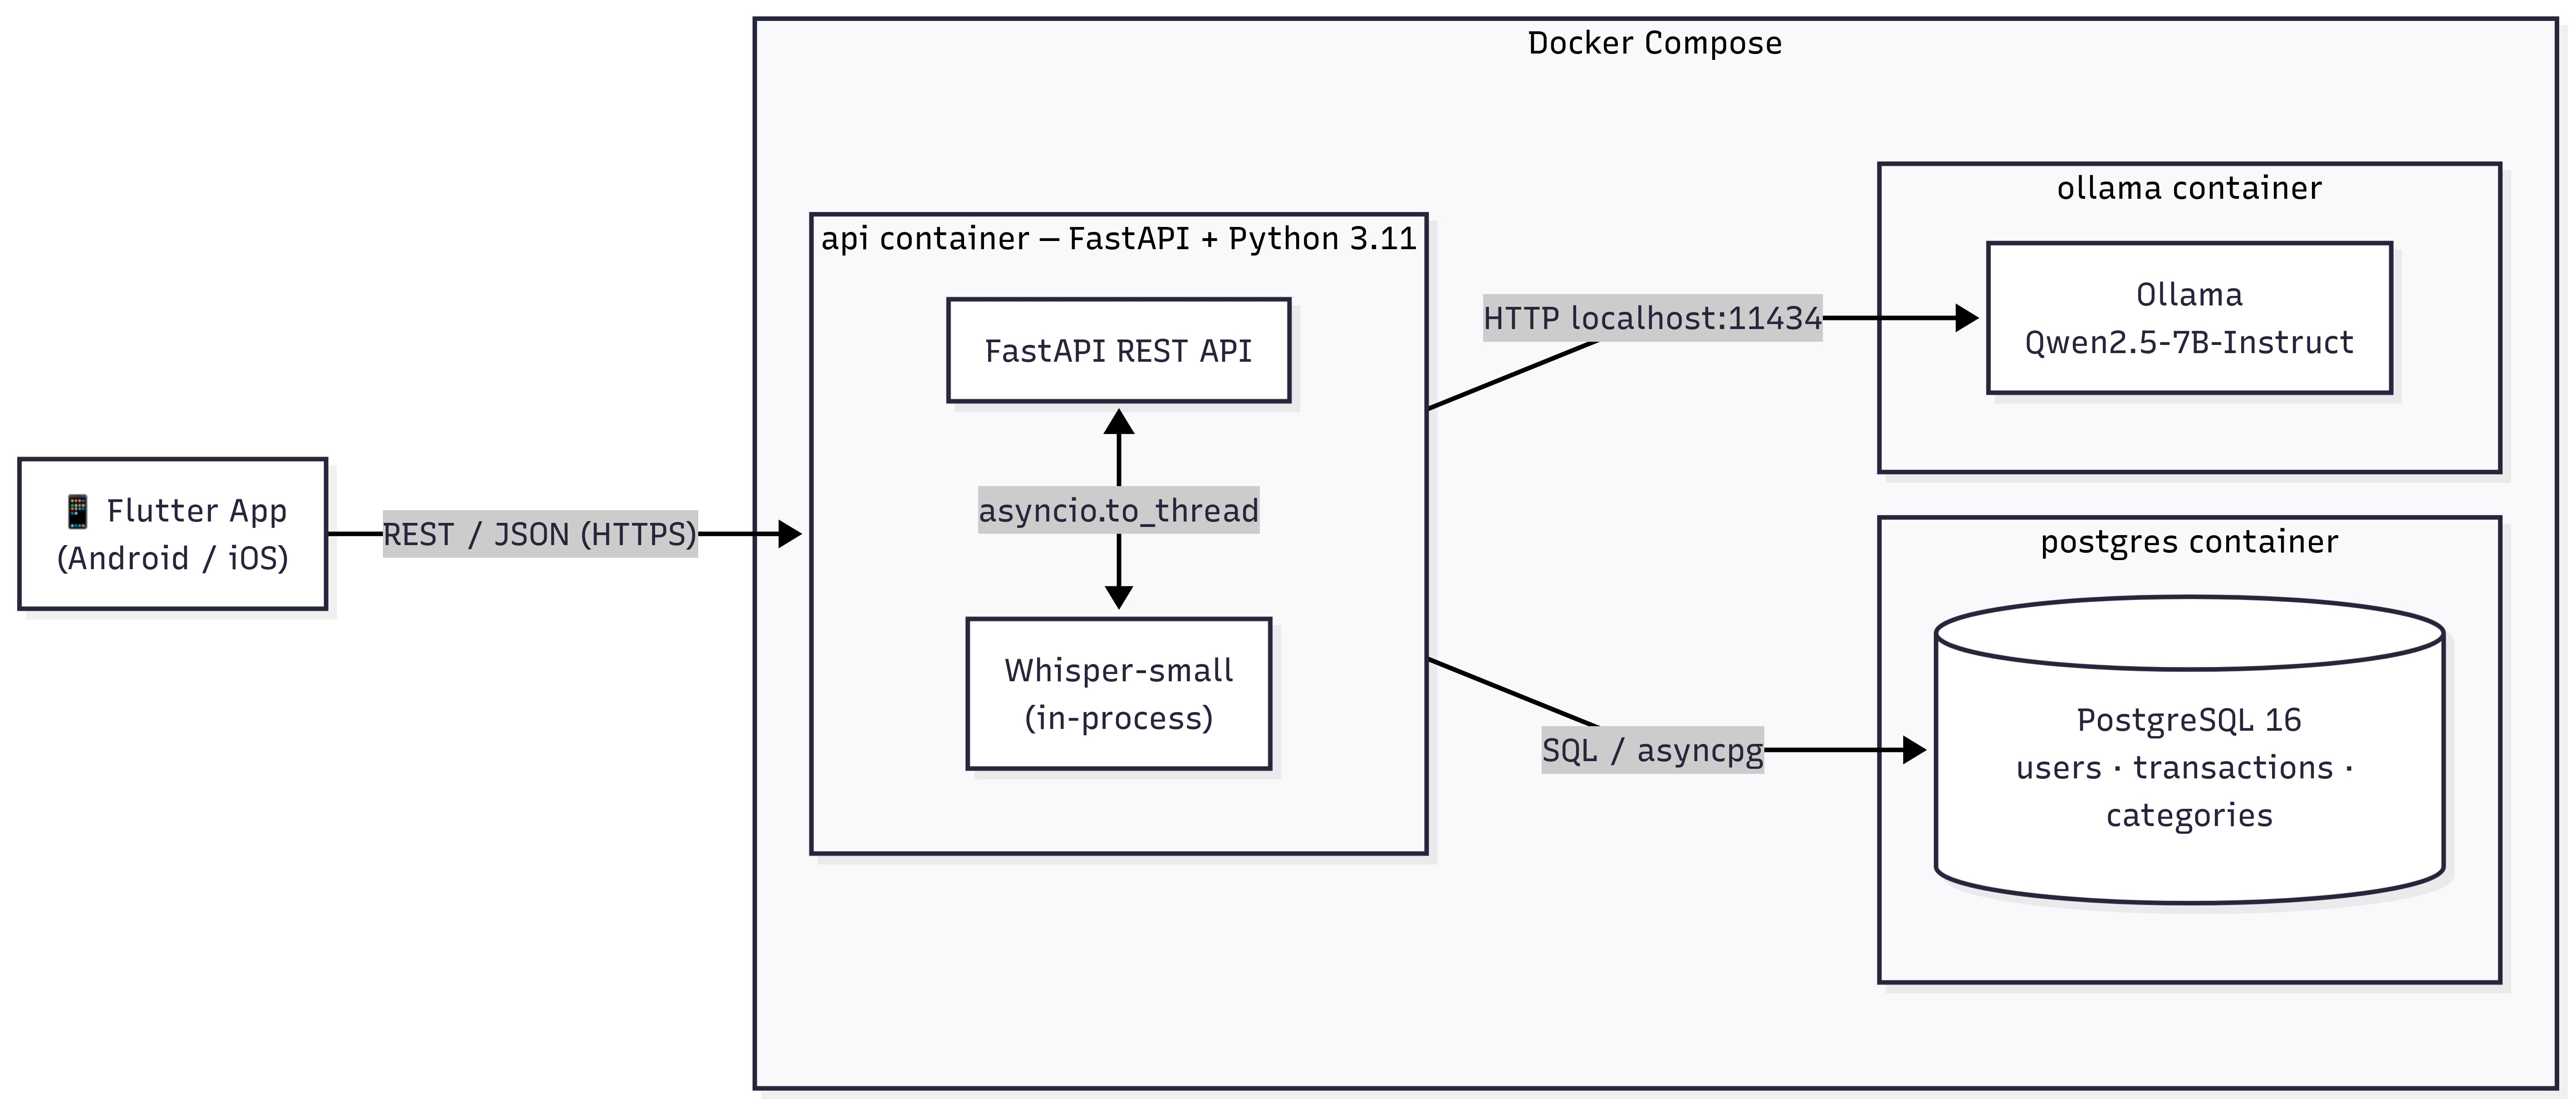
\includegraphics[width=\textwidth]{figures/system_architecture.jpg}
    \caption[High-level system architecture]{High-level system architecture. The
    Flutter client communicates over REST/JSON with the FastAPI backend, which
    hosts the Whisper model in-process and calls the Ollama language-model server
    over HTTP; PostgreSQL stores users, transactions, and categories. Three
    containers (\texttt{api}, \texttt{postgres}, \texttt{ollama}) are orchestrated
    by Docker Compose.}
    \label{fig:architecture}
\end{figure}

\begin{figure}[H]
    \centering
    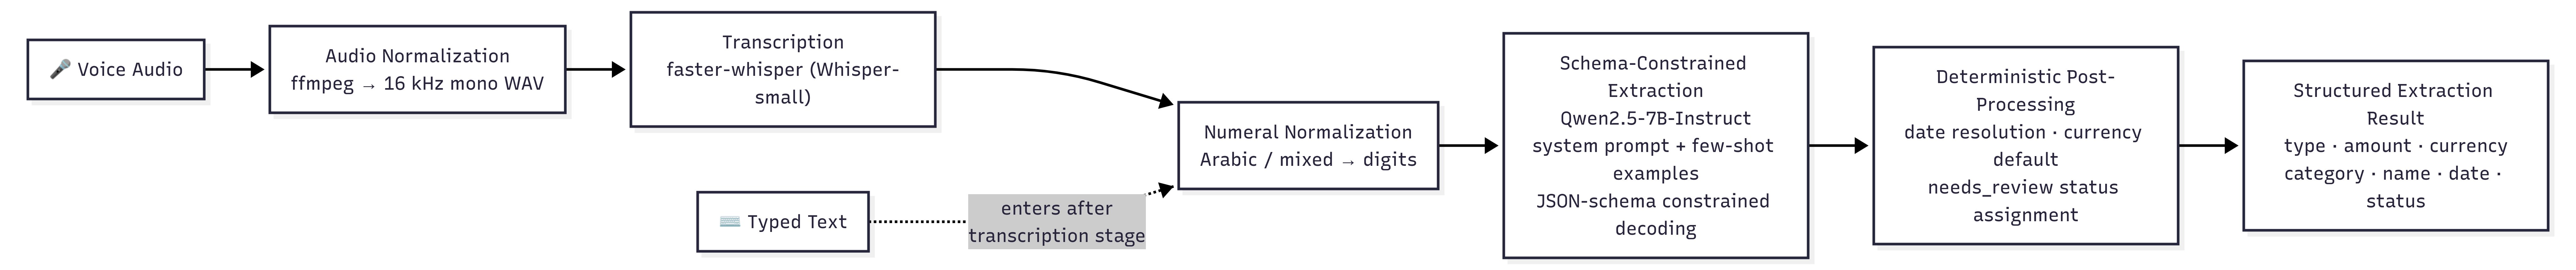
\includegraphics[width=\textwidth]{figures/ai_pipeline.jpg}
    \caption[The MiPay AI pipeline]{The MiPay AI pipeline. Audio is converted to
    16\,kHz mono WAV and transcribed by faster-whisper; the transcript is
    numeral-normalized and sent, with a fixed system prompt and few-shot examples,
    to the schema-constrained Qwen2.5-7B extractor; the deterministic
    post-processing layer resolves dates, fills defaults, and assigns each record a
    status. Text-mode input enters the same pipeline after the transcription
    stage.}
    \label{fig:pipeline}
\end{figure}

\subsection{Major Contributions of the Proposed System}

The implementation embodies four design decisions that distinguish it from a
naive cloud-API wrapper:

\begin{enumerate}[leftmargin=*]
    \item \textbf{Self-hosted open models.} Both the speech model and the language
    model run inside the deployment; no audio or text is sent to any third party,
    giving zero per-request cost and full data privacy.
    \item \textbf{Constrained decoding.} The language model is invoked with a JSON
    schema that the decoder is forced to satisfy, so output is always
    parseable and enum fields are always legal.
    \item \textbf{Hybrid fuzzy/exact division of labor.} The model performs
    language understanding; a deterministic, unit-tested layer performs the exact
    operations (numerals, dates, currency, status) the model does unreliably.
    \item \textbf{Stateless, human-in-the-loop pipeline.} The extraction endpoints
    persist nothing; records are saved only after explicit user confirmation,
    making any extraction error harmless and recoverable.
\end{enumerate}

\section{Proposed System Components}

\subsection{Component A --- Speech-to-Text Service}

\subsubsection{Notations}

Let an input audio clip be $x$, sampled and resampled to 16\,kHz mono. The
speech model defines a function
\[
\text{STT}(x) = (\hat{t},\; \ell,\; p_\ell),
\]
where $\hat{t}$ is the transcript, $\ell$ is the detected language, and
$p_\ell \in [0,1]$ is the language-identification probability. Whisper computes a
log-Mel spectrogram $M(x)$ and models
\[
\hat{t} = \arg\max_{t} \; \prod_{i=1}^{|t|} P_\theta\!\left(t_i \mid t_{<i},\, \text{Enc}_\theta(M(x))\right),
\]
approximated with beam search of width $5$.

\subsubsection{Methodology}

Transcription uses Whisper~\cite{radford2023whisper} served through
\texttt{faster-whisper}~\cite{fasterwhisper}, which executes the same weights on
the CTranslate2 engine~\cite{ctranslate2} with 8-bit
quantization~\cite{dettmers2022llmint8} for roughly a four-fold CPU speedup at
negligible accuracy cost. The model is loaded \emph{once} at application startup
via the FastAPI lifespan handler and held as a singleton; loading per request
would dominate latency. The default size is \texttt{small} (a good
Arabic/English balance on CPU), configurable to \texttt{base} or \texttt{medium}
through an environment variable. Three decoding choices matter for this domain:
language is left to \emph{auto-detection} (\texttt{language=None}), which is
essential for Arabic, English, and code-switched clips; beam search width is
$5$; and a voice-activity-detection filter trims silence, which markedly improves
accuracy on short clips and suppresses the hallucinated text Whisper can emit
during long silences. Listing~\ref{lst:stt} shows the core service.

\begin{lstlisting}[language=Python, caption={The speech-to-text service (\texttt{app/services/stt.py}).}, label={lst:stt}]
class STTService:
    def __init__(self) -> None:
        self._model = WhisperModel(
            settings.WHISPER_MODEL,            # "small" by default
            compute_type=settings.WHISPER_COMPUTE_TYPE,  # int8 on CPU
        )

    def transcribe(self, wav_path: Path) -> STTResult:
        segments, info = self._model.transcribe(
            str(wav_path),
            language=None,    # auto-detect: critical for ar/en/code-switching
            beam_size=5,
            vad_filter=True,  # trims silence; improves short-clip accuracy
        )
        transcript = " ".join(s.text for s in segments).strip()
        return STTResult(
            transcript=transcript,
            language=info.language,
            language_probability=info.language_probability,
        )
\end{lstlisting}

Audio handling enforces the privacy requirement (NFR-04): incoming
\texttt{m4a}/\texttt{aac}/\texttt{wav}/\texttt{mp3} is converted to 16\,kHz mono
WAV with \texttt{ffmpeg}, transcribed, and then \emph{immediately deleted}; the
transcription call runs in a worker thread (\texttt{asyncio.to\_thread}) so the
event loop stays responsive during the CPU-bound decode.

\subsection{Component B --- Constrained LLM Extraction}
\label{sec:ch4-extraction}

\subsubsection{Key Responsibilities}

The extractor converts a transcript into a list of structured transaction
objects. It must (i) understand intent across Arabic, English, and mixed input;
(ii) split compound utterances into separate transactions; (iii) map spoken
currency and category words onto fixed enumerations; and (iv) return output that
is \emph{guaranteed} machine-parseable.

\subsubsection{Feature Representation: the Extraction Schema}
\label{sec:ch4-schema}

A single utterance may describe several transactions, so the model returns a
list of per-transaction objects under a \texttt{transactions} key. Each object
has seven fields, three of which are constrained to enumerations
(\texttt{transaction\_type}, \texttt{currency}, \texttt{category}).
Listing~\ref{lst:schema} shows the per-item schema sent to the model.

\begin{lstlisting}[language=Python, caption={The per-transaction extraction schema (excerpt of \texttt{app/services/extraction.py}).}, label={lst:schema}]
TRANSACTION_ITEM_SCHEMA = {
  "type": "object",
  "properties": {
    "transaction_type": {"type": ["string","null"],
                         "enum": ["expense","income",None]},
    "amount":   {"type": ["number","null"]},
    "currency": {"type": ["string","null"],
                 "enum": ["SAR","USD","EUR","EGP","AED","KWD","QAR","BHD",
                          "OMR","JOD","IQD","SYP","YER","LYD","TND","DZD",
                          "MAD","SDG","LBP",None]},
    "category": {"type": ["string","null"],
                 "enum": ["groceries","restaurants","transport","fuel",
                          "shopping","bills","rent","health","education",
                          "entertainment","travel","personal_care",
                          "gifts_donations","salary","business",
                          "transfer_in","other","coffee","internet_mobile",
                          "subscriptions","household","tuition","clothes",
                          "pets","insurance","savings","transfer_out",
                          "freelance","investments",None]},
    "name":       {"type": ["string","null"]},
    "date_text":  {"type": ["string","null"]},
    "confidence": {"type": "string", "enum": ["high","medium","low"]},
  },
  "required": ["transaction_type","amount","currency","category",
               "name","date_text","confidence"],
}
\end{lstlisting}

A subtle but important design point is the \texttt{date\_text} field: the model
is asked to copy the \emph{raw} date phrase from the utterance (``yesterday'',
``last Friday'', the Arabic ``\emph{ams}'') and explicitly \emph{not} to resolve
it to a calendar date. Date arithmetic is delegated to deterministic code
(Component~C), because language models are unreliable at
it~\cite{qwen2024qwen25} and a deterministic resolver is independently testable.

\subsubsection{Processing Pipeline: Prompt and Constrained Decoding}

Extraction is a single chat completion against the Ollama
server~\cite{ollama2024} hosting Qwen2.5-7B-Instruct~\cite{qwen2024qwen25}. Three
elements make it reliable. First, a detailed \textbf{system prompt} specifies the
field rules---how to decide expense versus income, how to convert spelled-out
numbers in either language, how to disambiguate currencies by national context,
and how to map merchant words to categories. Second, a sequence of
\textbf{few-shot examples}~\cite{brown2020gpt3} is sent as alternating
user/assistant messages; these teach the model to wrap output in the
\texttt{transactions} list, to split compound utterances, and to return an empty
list when no transaction is present. Third, and decisively, the request sets
\texttt{format} to the JSON schema and \texttt{temperature} to $0$, so decoding is
both \textbf{deterministic} and \textbf{schema-constrained}: every token that
would break the schema is masked out at generation
time~\cite{willard2023outlines,geng2023grammar}. Listing~\ref{lst:extract} shows
the call.

\begin{lstlisting}[language=Python, caption={The constrained extraction call (\texttt{app/services/extraction.py}).}, label={lst:extract}]
payload = {
    "model": settings.EXTRACTION_MODEL,        # qwen2.5:7b-instruct
    "messages": _build_messages(transcript),   # system + few-shots + transcript
    "format": EXTRACTION_SCHEMA,   # constrained decoding -> valid JSON guaranteed
    "options": {"temperature": 0},             # deterministic extraction
    "stream": False,
}
async with httpx.AsyncClient(timeout=httpx.Timeout(180.0, connect=5.0)) as client:
    response = await client.post(f"{settings.OLLAMA_URL}/api/chat", json=payload)
    response.raise_for_status()
    content = response.json()["message"]["content"]
    return json.loads(content)   # always parseable thanks to constrained decoding
\end{lstlisting}

\subsubsection{Output Specification}

The call returns a dictionary with a \texttt{transactions} array; each element
conforms to Listing~\ref{lst:schema}. Because decoding is constrained, the
application never needs a JSON-repair or retry path for malformed output---an
entire class of failures common to prompt-only JSON generation is eliminated by
construction. If the Ollama server is unreachable or returns a transport error,
the call raises a typed \texttt{ExtractionError} that the API surfaces as a
\texttt{502 EXTRACTION\_FAILED}, prompting the client to offer manual entry.

\subsection{Component C --- Deterministic Post-Processing}

\subsubsection{Methodology and Implementation}

The post-processing layer is the deterministic counterpart to the fuzzy LLM. It
is the most heavily unit-tested module in the codebase, and it performs six
operations per the project specification, each idempotent and side-effect-free.

\paragraph{(1) Validation.} Each raw object is parsed into a Pydantic model
mirroring the schema; a parse failure (which constrained decoding should make
impossible) causes the item to be dropped rather than crash the request.

\paragraph{(2) Arabic-Indic numeral normalization.} A character-level
translation maps Eastern Arabic digits to Western digits and the Arabic decimal
separator to a period. This is applied to the transcript \emph{before} the model
sees it and to the \texttt{name} field afterward, so amounts and names are
consistent regardless of how the user spoke or the model wrote them.

\paragraph{(3) Date resolution.} The raw \texttt{date\_text} is resolved to an
absolute date anchored on the device's current date. The implementation first
maps dialectal Arabic phrases that the general parser misses
(e.g., several spellings of ``yesterday'' and ``the day before yesterday'') onto
canonical phrases, then calls the \texttt{dateparser}
library~\cite{dateparser} with the anchor as the relative base and a
``prefer past'' setting; a small set of retry transforms handles weekday phrases.
A null or unparseable phrase falls back to the anchor date.
Listing~\ref{lst:dates} shows the resolver.

\begin{lstlisting}[language=Python, caption={Deterministic relative-date resolution (\texttt{app/services/postprocess.py}).}, label={lst:dates}]
def resolve_date(date_text: str | None, client_date: date_type) -> date_type:
    if not date_text or not date_text.strip():
        return client_date

    phrase = normalize_numerals(date_text.strip())
    phrase = _DIALECT_DATE_MAP.get(phrase, phrase)   # dialect -> canonical phrase

    anchor = datetime(client_date.year, client_date.month, client_date.day)
    settings = {"RELATIVE_BASE": anchor, "PREFER_DATES_FROM": "past"}

    resolved = dateparser.parse(phrase, languages=["ar", "en"], settings=settings)
    if resolved is None:                 # retry: strip "yom"/"last", map "qabl"
        retry = phrase.lower()
        for pattern, replacement in _RETRY_TRANSFORMS:
            retry = pattern.sub(replacement, retry)
        if retry != phrase.lower():
            resolved = dateparser.parse(retry, languages=["ar","en"], settings=settings)

    return resolved.date() if resolved else client_date
\end{lstlisting}

\paragraph{(4) Currency defaulting.} A null currency is filled from the user's
profile default (e.g., \texttt{EGP}, the system default for Egyptian users).

\paragraph{(5) Category guard.} If the category is null but a transaction type is
present, the category is set to \texttt{other} so the record is never
category-less.

\paragraph{(6) Status decision.} Each surviving record is labeled \texttt{ok}
when both its type and amount are present and confidence is not low, otherwise
\texttt{needs\_review}. At the utterance level, the status is \texttt{failed} if
the transcript was empty or no record survived, \texttt{needs\_review} if any
record needs review, and \texttt{ok} otherwise. Junk objects in which both type
and amount are null are dropped so they never become blank confirmation cards.

\subsubsection{Evaluation and Results}

Because this layer is deterministic, it is validated by unit tests rather than by
statistical evaluation: the test suite covers numeral normalization, each dialect
date mapping, the weekday retry transforms, currency defaulting, the category
guard, and every branch of the status decision. This testability is itself an
argument for the hybrid design: the parts of the system that must be
\emph{exactly} correct are the parts that are deterministic and tested, while the
parts that are inherently fuzzy are bounded by constrained decoding and human
confirmation. The statistical evaluation of the fuzzy components is the subject
of Chapter~5.

\section{Pipeline Orchestration and Backend}

\subsection{Two Entry Points, One Core}

The orchestrator exposes \texttt{process\_audio} (voice mode) and
\texttt{process\_text} (text mode), both delegating to a shared
\texttt{\_extract\_and\_post} core that normalizes numerals, calls the extractor,
post-processes every returned record, and computes the utterance status and
timing. This structure is what makes the typed-text input mode (FR-14) almost
free: it reuses the entire extraction and post-processing path, simply skipping
the speech stage. Listing~\ref{lst:pipeline} shows the shared core.

\begin{lstlisting}[language=Python, caption={The shared extraction core (\texttt{app/services/voice\_pipeline.py}).}, label={lst:pipeline}]
async def _extract_and_post(transcript, client_date, default_currency,
                            detected_language, stt_ms, start):
    transcript = normalize_numerals(transcript).strip()
    if not transcript:
        return PipelineResult(status="failed", transcript="", ...)

    raw = await extraction_svc.extract(transcript)          # constrained LLM call
    raw_transactions = raw.get("transactions", [])
    results = postprocess_many(raw_transactions, client_date, default_currency)
    items = [PipelineItem(status=r.status, extraction=r.extraction)
             for r in results if r.extraction is not None]

    if not items:
        status = "failed"
    elif any(it.status == "needs_review" for it in items):
        status = "needs_review"
    else:
        status = "ok"
    return PipelineResult(status=status, transcript=transcript,
                          detected_language=detected_language, items=items, ...)
\end{lstlisting}

\subsection{REST API and Two-Step Save}

The backend exposes a versioned REST API (prefix \texttt{/api/v1}) built on
FastAPI~\cite{fastapi} with async SQLAlchemy~\cite{sqlalchemy} over
PostgreSQL~\cite{postgresql}. Table~\ref{tab:endpoints} lists the principal
endpoints. The architectural keystone is the \emph{two-step save}: the voice and
text endpoints return an extraction but \emph{persist nothing}; the client saves
the user-confirmed records through a separate batch endpoint. This keeps the AI
pipeline stateless, makes wrong extractions harmless, and provides the natural
human-in-the-loop checkpoint.

\begin{table}[H]
\centering
\caption{Principal API endpoints (all under \texttt{/api/v1}; all transaction, category, and summary routes require authentication).}
\label{tab:endpoints}
\small
\renewcommand{\arraystretch}{1.2}
\begin{tabularx}{\textwidth}{l l X}
\toprule
\textbf{Method} & \textbf{Path} & \textbf{Purpose} \\
\midrule
POST & \texttt{/auth/register} & Create a user; return token pair. \\
POST & \texttt{/auth/login} & Authenticate; return token pair. \\
POST & \texttt{/auth/refresh} & Rotate and reissue tokens. \\
POST & \texttt{/transactions/voice} & Audio in $\rightarrow$ extraction out; saves nothing. \\
POST & \texttt{/transactions/extract-text} & Text in $\rightarrow$ extraction out; saves nothing. \\
POST & \texttt{/transactions} & Create one transaction. \\
POST & \texttt{/transactions/batch} & Create many atomically (multi-transaction save). \\
GET & \texttt{/transactions} & List, filter, paginate. \\
PATCH/DELETE & \texttt{/transactions/\{id\}} & Edit / delete. \\
GET & \texttt{/categories} & Bilingual category reference list. \\
GET & \texttt{/summary} & Monthly totals and per-category breakdown. \\
GET & \texttt{/health} & Liveness of Whisper, Ollama, and the database. \\
\bottomrule
\end{tabularx}
\end{table}

\subsection{Security Model}

Authentication uses JSON Web Tokens signed with HS256: a short-lived access token
(30 minutes) and a long-lived refresh token (30 days) that is rotated on every
refresh. A \texttt{token\_version} integer on the user row is embedded in refresh
tokens so that ``log out everywhere'' is a single increment. Passwords are hashed
with bcrypt. Every transaction and summary query is filtered by the authenticated
user's identifier, enforcing per-user data isolation server-side (FR-13), and a
global exception handler renders all errors in the uniform
\texttt{\{error:\{code,message\}\}} envelope (NFR-05). These mechanisms are
detailed further in Appendix~A.

\section{Domain Reference Data}

Three fixed vocabularies anchor the extraction schema and the database: the
category taxonomy, the supported currencies, and the API error codes. They are
reproduced here because they define the closed sets the constrained decoder is
permitted to emit and the contract the client programs against.

\subsection{Category Taxonomy}

The twenty-nine categories (Table~\ref{tab:categories}) are seeded into the
database with bilingual Egyptian-Arabic labels and a Material icon name; the
language model's \texttt{category} field is constrained to exactly these keys
plus \texttt{null}. The original seventeen were extended by twelve
Egypt-relevant categories covering everyday spending patterns such as
mobile/internet recharges, café culture, subscriptions, gam'eya savings
circles, and freelance income.

\begin{table}[H]
\centering
\caption{The twenty-nine-category taxonomy (key, English label, kind).}
\label{tab:categories}
\small
\renewcommand{\arraystretch}{1.15}
\begin{tabular}{lll|lll}
\toprule
\textbf{Key} & \textbf{Label} & \textbf{Kind} & \textbf{Key} & \textbf{Label} & \textbf{Kind} \\
\midrule
groceries      & Groceries       & expense & education       & Education       & expense \\
restaurants    & Restaurants     & expense & entertainment   & Entertainment   & expense \\
transport      & Transport       & expense & travel          & Travel          & expense \\
fuel           & Fuel            & expense & personal\_care   & Personal Care   & expense \\
shopping       & Shopping        & expense & gifts\_donations & Gifts/Donations & expense \\
bills          & Bills           & expense & salary          & Salary          & income \\
rent           & Rent            & expense & business        & Business        & both \\
health         & Health          & expense & transfer\_in     & Transfer In     & income \\
other          & Other           & both    & coffee          & Coffee \& Cafés & expense \\
internet\_mobile & Internet \& Mobile & expense & subscriptions & Subscriptions   & expense \\
household      & Home \& Family  & expense & tuition         & Private Lessons & expense \\
clothes        & Clothes         & expense & pets            & Pets            & expense \\
insurance      & Insurance       & expense & savings         & Savings/Gam'eya & both \\
transfer\_out  & Transfer Out    & expense & freelance       & Freelance       & income \\
investments    & Investments     & both    &                 &                 & \\
\bottomrule
\end{tabular}
\end{table}

\subsection{Supported Currencies}

The \texttt{currency} field is constrained to nineteen ISO~4217 codes covering the
Arab region plus the major reserve currencies (Table~\ref{tab:currencies}). The
prompt encodes the disambiguation rules (for example, ``dinar'' resolves to KWD,
JOD, BHD, IQD, LYD, or TND according to national context), and a null currency is
filled from the user's profile default during post-processing.

\begin{table}[H]
\centering
\caption{Supported ISO 4217 currency codes.}
\label{tab:currencies}
\small
\renewcommand{\arraystretch}{1.15}
\begin{tabularx}{\textwidth}{X X X X X}
\toprule
SAR (Saudi) & USD (US) & EUR (Euro) & EGP (Egypt) & AED (UAE) \\
KWD (Kuwait) & QAR (Qatar) & BHD (Bahrain) & OMR (Oman) & JOD (Jordan) \\
IQD (Iraq) & SYP (Syria) & YER (Yemen) & LYD (Libya) & TND (Tunisia) \\
DZD (Algeria) & MAD (Morocco) & SDG (Sudan) & LBP (Lebanon) & \\
\bottomrule
\end{tabularx}
\end{table}

\subsection{API Error Codes}

All failures are returned in the uniform \texttt{\{error:\{code,message\}\}}
envelope; Table~\ref{tab:errors} lists the codes the client handles. Mapping
each to a specific user experience (for example, \texttt{EXTRACTION\_FAILED}
offers manual entry) is what makes the system degrade gracefully rather than
crash.

\begin{table}[H]
\centering
\caption{API error codes and their HTTP status.}
\label{tab:errors}
\small
\renewcommand{\arraystretch}{1.2}
\begin{tabularx}{\textwidth}{l c X}
\toprule
\textbf{Code} & \textbf{HTTP} & \textbf{Meaning / client behavior} \\
\midrule
\texttt{VALIDATION\_ERROR}   & 422 & Malformed input; show field errors. \\
\texttt{INVALID\_CREDENTIALS}& 401 & Wrong email/password on login. \\
\texttt{TOKEN\_EXPIRED}      & 401 & Triggers the silent refresh-and-retry path. \\
\texttt{NOT\_FOUND}          & 404 & Resource absent or not owned by the user. \\
\texttt{AUDIO\_TOO\_LONG}    & 413 & Clip exceeds the 30-second limit. \\
\texttt{AUDIO\_UNSUPPORTED}  & 415 & Unsupported audio format. \\
\texttt{EXTRACTION\_FAILED}  & 502 & Ollama unreachable; offer manual entry. \\
\texttt{INTERNAL}            & 500 & Unexpected error; generic message. \\
\bottomrule
\end{tabularx}
\end{table}

\subsection{A Worked End-to-End Example}

To make the pipeline concrete, consider the multi-transaction utterance
``\,I bought a coffee for 50 and a croissant for 100 and my father gave me
200\,'' spoken on 15 June 2026. The stages transform it as follows:

\begin{enumerate}[leftmargin=*]
    \item \textbf{Transcription} yields the transcript text and a detected language
    of \texttt{en} with high probability.
    \item \textbf{Numeral normalization} is a no-op here (Western digits already).
    \item \textbf{Constrained extraction} returns a \texttt{transactions} array of
    \emph{three} objects: two expenses (\texttt{restaurants}, amounts 50 and 100)
    and one income (\texttt{transfer\_in}, amount 200, name ``father''), each with
    \texttt{date\_text} null and confidence high.
    \item \textbf{Post-processing} resolves each null \texttt{date\_text} to the
    anchor date 2026-06-15, fills the null currency from the profile default,
    keeps every category, and assigns each record status \texttt{ok}.
    \item \textbf{Pipeline} reports a top-level status of \texttt{ok}, transaction
    count three, and per-stage timing.
    \item \textbf{Client} renders three editable cards; on confirmation the app
    calls the batch endpoint, which inserts all three atomically.
\end{enumerate}

This single example exercises multi-transaction splitting, type disambiguation
(expense versus income within one sentence), currency defaulting, and date
anchoring---the four behaviors that distinguish the pipeline from a naive
single-field parser.

\section{Mobile Client}

The client is a Flutter~\cite{flutter} application using Riverpod~\cite{riverpod}
for state management, Dio for HTTP with an interceptor that transparently
attaches and refreshes tokens, and \texttt{flutter\_secure\_storage} for token
persistence. The recording flow is modeled as an explicit state machine
(\texttt{idle} $\rightarrow$ \texttt{recording} $\rightarrow$ \texttt{uploading}
$\rightarrow$ \texttt{processing} $\rightarrow$ \texttt{result}\,$\mid$\,\texttt{error}),
which drives the staged progress UI (``Transcribing\ldots'' then
``Analyzing\ldots''). The interface is fully localized through ARB files for
Arabic (Egyptian dialect) and English; switching language flips the entire app,
including right-to-left layout, instantly. The confirmation screen renders one
editable card per extracted record, tinting \texttt{needs\_review} cards, and
commits all records through the atomic batch endpoint.

\textbf{Cross-user data isolation.} Every per-user Riverpod provider
(\texttt{transactionsProvider}, \texttt{summaryProvider},
\texttt{recordingControllerProvider}) watches a \texttt{currentUserIdProvider}
derived from the authentication state. When the authenticated user changes
(login, logout, or session expiry), Riverpod automatically tears down and
rebuilds all dependent providers, making it structurally impossible for user
A's cached data to remain in memory when user B signs in.

\textbf{Design system.} The foundation is a hand-built \texttt{ColorScheme}---
ink-black (\texttt{\#0B0B0D}) on white in light mode, near-white on
\texttt{\#0B0B0D} in dark mode---with no Material seed color, plus a
\texttt{ThemeExtension} (\texttt{AppSemanticColors}) that confines green/red to
income/expense amounts. On top of this neutral base, a brand gradient
(indigo\,$\rightarrow$\,violet) drives the dashboard's balance hero card and
primary call-to-action buttons, and a deterministic hash from category key to
a fixed sixteen-color palette (\texttt{categoryColor()}) gives every category
a stable, hue-distinct color reused consistently across the donut chart, the
category breakdown list, transaction tiles, and filter chips---replacing an
earlier grayscale-only chart palette. A three-way appearance toggle (system /
light / dark) is stored in \texttt{SharedPreferences} and loaded before
\texttt{runApp} to eliminate any theme flash on launch.

The user-interface gallery is presented in Appendix~A.

\section{Deployment}

The system is delivered as three Docker Compose services---\texttt{api} (FastAPI
with Whisper in-process and \texttt{ffmpeg} available), \texttt{postgres}, and
\texttt{ollama}---with persistent volumes for the database, the Ollama model
store, and the cached Whisper weights. One-time provisioning pulls the language
model (\texttt{ollama pull qwen2.5:7b-instruct}) and applies database migrations.
The reference deployment runs entirely on a CPU-only 16\,GB machine; a GPU, if
present, is optional acceleration that enables the larger \texttt{medium} Whisper
model and faster language-model inference. This single-command reproducibility
(NFR-08) is what allows the evaluation in the next chapter to be repeated by a
third party.
